% chapter2.tex -- Preliminaries
% Based on UGThesis.docx and Parvez et al. 2011 paper.

\chapter{Preliminaries}
\label{ch:preliminaries}

In this chapter, we define the basic concepts used throughout the thesis. 
We assume the reader is familiar with elementary graph theory, but we provide precise definitions to avoid ambiguity. 
Special emphasis is given to notions that are essential for biconnected plane graphs, such as separation pairs and separation vertices, which do not appear in the triconnected case.

\section{Basic Graph Definitions}
\label{sec:basic_graph_defs}

Let \(G = (V, E)\) be a connected simple graph with vertex set \(V\) and edge set \(E\). 
Each edge \(e \in E\) is an unordered pair \(\{u, v\}\) with \(u, v \in V\) and \(u \neq v\). 
We denote an edge between \(u\) and \(v\) by \((u, v)\) or \((v, u)\).

The \textbf{degree} of a vertex \(v\) is the number of edges incident to \(v\). 
A graph is \textbf{simple} if it has no loops or multiple edges.

The \textbf{connectivity} \(\kappa(G)\) of a graph \(G\) is the minimum number of vertices whose removal disconnects the graph (or reduces it to a single vertex). 
A graph is \textbf{\(k\)-connected} if \(\kappa(G) \ge k\). 
Equivalently, removing fewer than \(k\) vertices leaves the graph connected.

In particular:
\begin{itemize}
    \item A graph is \textbf{2-connected} (or \textbf{biconnected}) if it has no articulation vertices (cut vertices) and remains connected after the removal of any single vertex.
    \item A graph is \textbf{3-connected} (or \textbf{triconnected}) if it remains connected after the removal of any two vertices.
\end{itemize}

\begin{definition}[Separation pair]
    \label{def:separation_pair}
    In a biconnected graph, a pair of vertices \(\{a, b\}\) is called a \textbf{separation pair} if removing \(a\) and \(b\) disconnects the graph into at least two components. 
    A biconnected graph that contains a separation pair is not triconnected.
\end{definition}

\begin{definition}[Separation vertex]
    \label{def:separation_vertex}
    In a 1-connected graph, a vertex \(v\) is a \textbf{separation vertex} (or \textbf{cut vertex}) if removing \(v\) disconnects the graph. 
    A graph is biconnected if and only if it has no separation vertices.
\end{definition}

The distinction between biconnected and triconnected graphs is crucial: 
triconnected graphs have no separation pairs, while biconnected graphs may have them. 
The presence of separation pairs is the main obstacle when extending triangulation generation algorithms from triconnected to biconnected graphs.

\section{Planar and Plane Graphs}
\label{sec:planar_plane}

A graph \(G\) is \textbf{planar} if it can be drawn in the plane without any edge crossings. 
Such a drawing is called an \textbf{embedding}. 
A \textbf{plane graph} is a planar graph together with a fixed embedding in the plane.

A plane graph divides the plane into connected regions called \textbf{faces}. 
The unbounded region is the \textbf{outer face}; all other faces are \textbf{inner faces}. 
Each face is bounded by a closed walk along the edges of the graph.

If every face boundary contains exactly three edges, the plane graph is called a \textbf{plane triangulation}. 
In this thesis, edges are not required to be straight lines; triangulation is understood combinatorially.

\section{Separation Pairs and Separation Vertices}
\label{sec:separation_pairs_vertices}

We now discuss separation pairs in more detail, as they are central to the biconnected case.

\begin{figure}[htbp]
    \centering
    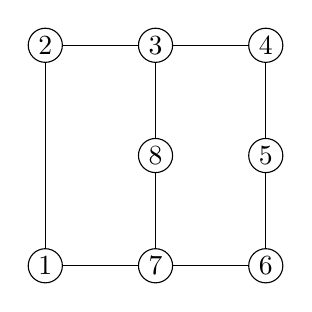
\begin{tikzpicture}[scale=0.7, every node/.style={circle, draw, fill=white, inner sep=1.5pt}]
        \coordinate (1) at (0,2);
        \coordinate (2) at (0,6);
        \coordinate (3) at (2,6);
        \coordinate (4) at (4,6);
        \coordinate (5) at (4,4);
        \coordinate (6) at (4,2);
        \coordinate (7) at (2,2);
        \coordinate (8) at (2,4);
        \draw (1)--(2)--(3)--(4)--(5)--(6)--(7)--(8);
        \draw (1)--(7);
        \draw (3)--(8);
        \node at (1) {1};
        \node at (2) {2};
        \node at (3) {3};
        \node at (4) {4};
        \node at (5) {5};
        \node at (6) {6};
        \node at (7) {7};
        \node at (8) {8};
    \end{tikzpicture}
    \caption{A biconnected plane graph. Vertices 3 and 7 form a separation pair.}
    \label{fig:separation_pair_example}
\end{figure}

Figure~\ref{fig:separation_pair_example} shows a biconnected plane graph with eight vertices. 
Removing vertices 3 and 7 disconnects the remaining vertices into three components: \(\{1,2\}\), \(\{4,5,6\}\), and \(\{8\}\). 
Therefore, \((3,7)\) is a separation pair.

\begin{remark}
    In a biconnected plane graph, a separation pair \((a,b)\) implies that the graph can be split into two subgraphs that share only \(a\) and \(b\). 
    Consequently, there exist two faces (one on each side of the pair) that can potentially contain the same chord \((a,b)\), leading to a multi-edge if both faces are triangulated independently.
\end{remark}

\section{Faces, Cycles, and Chords}
\label{sec:faces_cycles_chords}

A \textbf{cycle} \(C\) in a graph is a sequence of distinct vertices \(v_1, v_2, \ldots, v_k\) such that \((v_i, v_{i+1}) \in E\) for \(1 \le i < k\) and \((v_k, v_1) \in E\). 
In a plane graph, each face corresponds to a cycle that bounds it (taking the outer face as a cycle as well).

Let \(C = \langle v_1, v_2, \ldots, v_n \rangle\) be a cycle, listed in counterclockwise order. 
An edge \((v_i, v_j)\) is called a \textbf{chord} of \(C\) if it is not an edge of \(C\) and its interior lies inside the face bounded by \(C\). 
A chord \((v_i, v_j)\) divides the cycle into two smaller cycles: 
\(v_i, v_{i+1}, \ldots, v_j\) and \(v_j, v_{j+1}, \ldots, v_i\).

\begin{figure}[htbp]
    \centering
    \begin{subfigure}{0.45\textwidth}
        \centering
        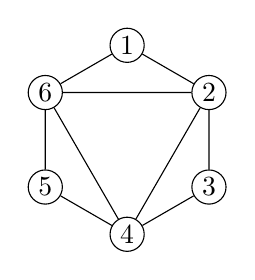
\begin{tikzpicture}[scale=0.8, every node/.style={circle, draw, fill=white, inner sep=1.5pt}]
            \foreach \i/\angle in {1/90,2/30,3/-30,4/-90,5/-150,6/150} {
                \node (v\i) at (\angle:1.5) {\i};
            }
            \draw (v1)--(v2)--(v3)--(v4)--(v5)--(v6)--(v1);
            \draw (v2)--(v4)--(v6)--(v2);
        \end{tikzpicture}
        \caption{A triangulation of a hexagon.}
        \label{fig:triangulation_hex1}
    \end{subfigure}
    \hfill
    \begin{subfigure}{0.45\textwidth}
        \centering
        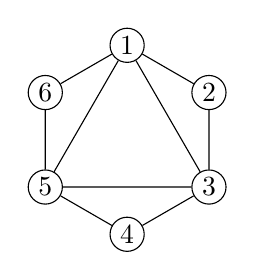
\begin{tikzpicture}[scale=0.8, every node/.style={circle, draw, fill=white, inner sep=1.5pt}]
            \foreach \i/\angle in {1/90,2/30,3/-30,4/-90,5/-150,6/150} {
                \node (v\i) at (\angle:1.5) {\i};
            }
            \draw (v1)--(v2)--(v3)--(v4)--(v5)--(v6)--(v1);
            \draw (v1)--(v3)--(v5)--(v1);
        \end{tikzpicture}
        \caption{Another triangulation of the same hexagon.}
        \label{fig:triangulation_hex2}
    \end{subfigure}
    \caption{Two different triangulations of a cycle with six vertices.}
    \label{fig:triangulations_of_cycle}
\end{figure}

\section{Triangulation of a Cycle}
\label{sec:triangulation_cycle}

A \textbf{triangulation} of a cycle \(C\) is a maximal set of non-intersecting chords that partition the interior of \(C\) into triangles. 
The sides of the triangles are either chords or edges of \(C\). 
Figure~\ref{fig:triangulations_of_cycle} shows two triangulations of a hexagon.

Equivalently, a triangulation of a cycle with \(n\) vertices contains exactly \(n-3\) chords. 
This follows from Euler’s formula applied to the planar graph formed by the cycle and its chords.

\section{Labeled vs. Unlabeled Triangulations}
\label{sec:labeled_unlabeled}

If the vertices of the cycle are numbered sequentially from \(v_1\) to \(v_n\), then a triangulation is called a \textbf{labeled triangulation}. 
The order of vertices matters: two triangulations that differ only by a rotation or reflection are considered distinct if the labels are different.

If the vertices are not numbered, the triangulations are called \textbf{unlabeled}. 
In this case, rotationally equivalent or mirror-image triangulations are considered the same. 
In this thesis, we work exclusively with \textbf{labeled triangulations} unless stated otherwise.

\section{Flipping Operation}
\label{sec:flipping_operation}

A fundamental operation for transforming one triangulation into another is the \textbf{flip}. 
Consider two adjacent triangles that share a chord and together form a quadrilateral. 
Removing the common chord and adding the opposite diagonal produces a new triangulation.

\begin{figure}[htbp]
    \centering
    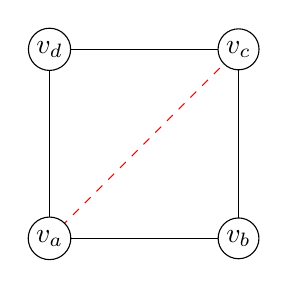
\begin{tikzpicture}[scale=1.2, every node/.style={circle, draw, fill=white, inner sep=1.5pt}]
        \coordinate (A) at (0,0);
        \coordinate (B) at (2,0);
        \coordinate (C) at (2,2);
        \coordinate (D) at (0,2);
        \draw (A)--(B)--(C)--(D)--cycle;
        \draw[dashed, red] (A)--(C);
        \node at (A) {\(v_a\)};
        \node at (B) {\(v_b\)};
        \node at (C) {\(v_c\)};
        \node at (D) {\(v_d\)};
    \end{tikzpicture}
    \qquad
    $\longrightarrow$
    \qquad
    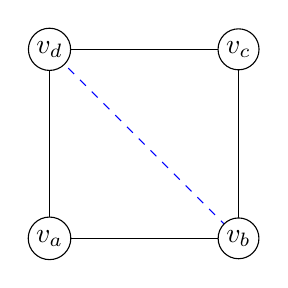
\begin{tikzpicture}[scale=1.2, every node/.style={circle, draw, fill=white, inner sep=1.5pt}]
        \coordinate (A) at (0,0);
        \coordinate (B) at (2,0);
        \coordinate (C) at (2,2);
        \coordinate (D) at (0,2);
        \draw (A)--(B)--(C)--(D)--cycle;
        \draw[dashed, blue] (B)--(D);
        \node at (A) {\(v_a\)};
        \node at (B) {\(v_b\)};
        \node at (C) {\(v_c\)};
        \node at (D) {\(v_d\)};
    \end{tikzpicture}
    \caption{Flipping the diagonal \((v_a, v_c)\) to \((v_b, v_d)\) in a quadrilateral.}
    \label{fig:flip_operation}
\end{figure}

Formally, let \((v_i, v_j)\) be a chord that belongs to two triangles \((v_i, v_j, v_p)\) and \((v_i, v_j, v_q)\) on opposite sides. 
These four vertices form a quadrilateral \(v_p, v_i, v_q, v_j\) in clockwise order. 
Flipping \((v_i, v_j)\) means removing it and adding the opposite chord \((v_p, v_q)\). 
The resulting graph is again a triangulation of the same cycle.

\section{Visibility, Blocking Chords, and Generating Chords}
\label{sec:visibility_blocking}

Fix a cycle \(C = \langle v_1, v_2, \ldots, v_n \rangle\) and choose a vertex, say \(v_1\), as the \textbf{root vertex}. 
In a triangulation \(T\) of \(C\), we say that a vertex \(v_j\) is \textbf{visible} from \(v_1\) if the chord \((v_1, v_j)\) belongs to \(T\).

In the root triangulation (the fan from \(v_1\)), every vertex except the neighbours \(v_2\) and \(v_n\) is visible from \(v_1\). 
In other triangulations, some vertices may be hidden behind \textbf{blocking chords}.

\begin{definition}[Blocking chord]
    \label{def:blocking_chord}
    A chord \((v_i, v_j)\) of a triangulation \(T\) is called a \textbf{blocking chord} if:
    \begin{enumerate}
        \item Neither \(v_i\) nor \(v_j\) is the root vertex \(v_1\), and
        \item The chord \((v_i, v_j)\) is visible from \(v_1\) in the sense that there is a triangle \((v_1, v_i, v_j)\) in \(T\).
    \end{enumerate}
    Equivalently, a blocking chord is a chord that does not have \(v_1\) as an endpoint but is directly connected to \(v_1\) via triangles.
\end{definition}

Blocking chords prevent some vertices from being visible from the root. 
Flipping a blocking chord replaces it with a chord that is incident to the root, thereby increasing the number of visible vertices.

\begin{definition}[Generating chord]
    \label{def:generating_chord}
    In a triangulation \(T\) of a cycle with root vertex \(v_1\), a chord \((v_1, v_j)\) is called a \textbf{generating chord} if flipping it produces a new triangulation \(T'\) whose leftmost blocking chord is exactly the newly added chord.
\end{definition}

The precise condition for a chord to be generating involves the leftmost blocking chord, which we define next.

\section{Leftmost Blocking Chord}
\label{sec:leftmost_blocking}

Among the blocking chords of a triangulation, we single out the one that is ``leftmost'' with respect to the cyclic order around the root.

\begin{definition}[Leftmost blocking chord]
    \label{def:leftmost_blocking}
    Let \(T\) be a triangulation of a cycle \(C = \langle v_1, v_2, \ldots, v_n \rangle\) with root vertex \(v_1\). 
    Let \((v_b, v_{b'})\) be a blocking chord of \(T\) with \(b < b'\). 
    It is the \textbf{leftmost blocking chord} if no other blocking chord \((v_i, v_j)\) satisfies \(j < b'\) (i.e., its larger index is smaller than \(b'\)). 
    In other words, among all blocking chords, the one with the smallest value of the larger endpoint is the leftmost.
\end{definition}

\begin{remark}
    The term ``leftmost'' comes from drawing the cycle with \(v_1\) at the top and the remaining vertices arranged clockwise around it. 
    Blocking chords then appear as chords that ``block'' the view to vertices on the left side.
\end{remark}

We now prove that the leftmost blocking chord is unique. 
The following argument is taken from the author’s original writing, polished for clarity.

\begin{lemma}[Uniqueness of the leftmost blocking chord]
    \label{lem:unique_leftmost}
    In any triangulation \(T\) of a cycle \(C = \langle v_1, v_2, \ldots, v_n \rangle\) that is not the root triangulation, there is exactly one leftmost blocking chord.
\end{lemma}

\begin{proof}
    Suppose, for contradiction, that there exist two distinct blocking chords that both qualify as leftmost. 
    Let the two chords be \((v_b, v_{b'})\) and \((v_c, v_{c'})\) with \(b < b'\) and \(c < c'\). 
    By definition of leftmost, we must have \(b' = c'\) (otherwise the one with the smaller larger endpoint would be unique). 
    Hence both chords share the same larger endpoint, say \(v_{b'} = v_{c'} = v_k\).

    Since both chords are blocking, each forms a triangle with the root vertex \(v_1\). 
    Thus we have triangles \((v_1, v_b, v_k)\) and \((v_1, v_c, v_k)\). 
    The vertices \(v_b\) and \(v_c\) lie on the same side of the chord \((v_1, v_k)\). 
    Without loss of generality, assume \(b < c\).

    Consider the quadrilateral formed by \(v_1, v_b, v_k, v_c\). 
    Because the triangulation is planar and all faces are triangles, the chord \((v_b, v_k)\) and \((v_c, v_k)\) cannot both be present without crossing. 
    In fact, only one of them can be a chord; the other must be replaced by the opposite diagonal of the quadrilateral. 
    However, if both are present, they would create a face with four vertices, contradicting that the triangulation is maximal. 
    Therefore, it is impossible to have two distinct blocking chords with the same larger endpoint. 
    Hence the leftmost blocking chord is unique.
\end{proof}

\begin{figure}[htbp]
    \centering
    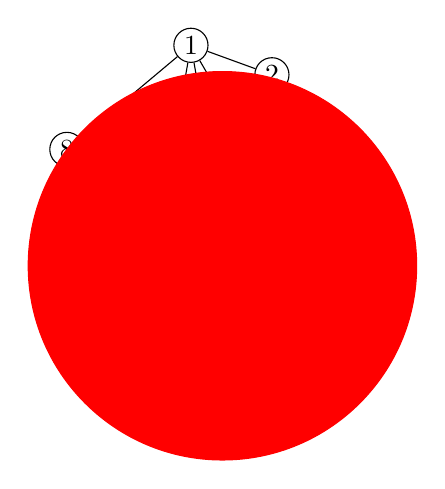
\begin{tikzpicture}[scale=0.8, every node/.style={circle, draw, fill=white, inner sep=1.5pt}]
        \foreach \i/\angle in {1/90,2/50,3/10,4/-30,5/-70,6/-110,7/-150,8/170} {
            \node (v\i) at (\angle:2) {\i};
        }
        \draw (v1)--(v2)--(v3)--(v4)--(v5)--(v6)--(v7)--(v8)--(v1);
        \draw (v1)--(v4);
        \draw (v1)--(v5);
        \draw (v1)--(v6);
        \draw[red, thick] (v4)--(v6);
        \node at (0,0) {\(v_1\)};
        \node[red] at (0.5, -1.5) {leftmost blocking chord \((v_4, v_6)\)};
    \end{tikzpicture}
    \caption{Illustration of the leftmost blocking chord. Here \((v_4, v_6)\) is the leftmost blocking chord because no other blocking chord has a larger endpoint smaller than 6.}
    \label{fig:leftmost_blocking}
\end{figure}

\section{Genealogical Tree of Triangulations}
\label{sec:genealogical_tree}

The parent–child relationship defined by flipping the leftmost blocking chord yields a rooted tree structure on the set of all triangulations of a cycle.

\begin{definition}[Genealogical tree]
    \label{def:genealogical_tree}
    Let \(C\) be a cycle with a fixed root vertex \(v_1\). 
    The \textbf{genealogical tree} \(\mathcal{T}(C)\) of triangulations of \(C\) is defined as follows:
    \begin{itemize}
        \item The root is the fan triangulation where all chords are incident to \(v_1\).
        \item For any non-root triangulation \(T\), its parent \(P(T)\) is obtained by flipping the leftmost blocking chord of \(T\).
        \item Conversely, a triangulation \(T\) is a child of \(T'\) if \(T' = P(T)\).
    \end{itemize}
\end{definition}

\begin{figure}[htbp]
    \centering
    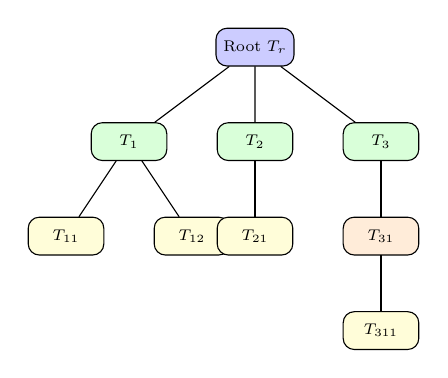
\begin{tikzpicture}[level distance=1.5cm, sibling distance=2cm, scale=0.8, transform shape]
        \tikzset{every node/.style={rectangle, draw, rounded corners, minimum width=1.2cm, minimum height=0.6cm, align=center, font=\scriptsize}}
        \node[fill=blue!20] {Root \(T_r\)}
            child { node[fill=green!15] {\(T_1\)}
                child { node[fill=yellow!15] {\(T_{11}\)} }
                child { node[fill=yellow!15] {\(T_{12}\)} }
            }
            child { node[fill=green!15] {\(T_2\)}
                child { node[fill=yellow!15] {\(T_{21}\)} }
            }
            child { node[fill=green!15] {\(T_3\)}
                child { node[fill=orange!15] {\(T_{31}\)}
                    child { node[fill=yellow!15] {\(T_{311}\)} }
                }
            };
    \end{tikzpicture}
    \caption{A schematic genealogical tree for a cycle. Each node represents a triangulation, and edges correspond to flipping a generating chord.}
    \label{fig:genealogical_tree}
\end{figure}

The genealogical tree has the following properties (proved in Chapter~\ref{ch:cycle_algorithm}):
\begin{itemize}
    \item Every triangulation appears exactly once.
    \item The root has \(n-3\) children (all chords are generating).
    \item The depth of the tree is at most \(n-2\).
    \item Flipping a generating chord takes constant time.
\end{itemize}

This tree structure is the basis of the algorithm for generating all triangulations of a cycle, which we recall in Chapter~\ref{ch:cycle_algorithm}.

\section{Summary}
\label{sec:prelim_summary}

We have introduced the essential graph-theoretic concepts: connectivity, planarity, faces, cycles, chords, triangulations, and the flipping operation. 
We defined blocking chords, generating chords, and the leftmost blocking chord, and proved its uniqueness. 
The genealogical tree provides a canonical parent–child relationship among triangulations of a cycle.

For biconnected graphs, we highlighted the significance of separation pairs, which are the main obstacle to extending the triconnected algorithm. 
These concepts will be used throughout the remainder of the thesis.